\documentclass[11pt,a4paper]{jlreq}
\usepackage{amsmath,amssymb}
\usepackage[dvipdfmx]{graphicx}
\usepackage{booktabs}
\usepackage{tikz}
\usetikzlibrary{arrows.meta,positioning}

\begin{document}

\begin{center}
{\LARGE \textbf{情報科学基礎A 第7回 レポート}}
\end{center}
\vspace{1em}

\begin{flushright}
提出日：\today \\
学籍番号：2611193 \\
氏名：中井平蔵
\end{flushright}

\section*{Assignment 1: 0-1 Knapsack Problem}

求める方法は様々あるが、動的計画法を用いる。

初めに、品物と添字 $i$の対応を示す。

\begin{table}[h]
\centering
\caption{品物と添字 $i$ の対応}
\begin{tabular*}{0.72\linewidth}{@{\extracolsep{\fill}}c|ccc@{}}
\toprule
 & i=0 (Orange) & i=1 (Banana) & i=2 (Apple) \\
\midrule
w & 2 & 3 & 4 \\
v & 6 & 7 & 8 \\
\bottomrule
\end{tabular*}
\end{table}

動的計画法の表は、各容量 $a$ に対して「その列の品物までを使ったときの最大価値」を表している。
最後に、$a=7$ かつ列 $i=0$ の値が最大価値となる。

\begin{table}[h]
\centering
\caption{動的計画法の表}
\begin{tabular*}{0.72\linewidth}{@{\extracolsep{\fill}}c|ccc@{}}
\toprule
 & i=2 & i=1 & i=0 \\
\midrule
a=1 & 0 & 0 & 0 \\
a=2 & 0 & 0 & 6 \\
a=3 & 0 & 7 & 7 \\
a=4 & \tikz[remember picture,baseline=(nA.base)]\node[inner sep=0pt,text=red] (nA) {8}; & 8 & 8 \\
a=5 & 8 & 8 & 13 \\
a=6 & 8 & 8 & 14 \\
a=7 & 8 & \tikz[remember picture,baseline=(nB.base)]\node[inner sep=0pt,text=red] (nB) {15}; & \tikz[remember picture,baseline=(nC.base)]\node[inner sep=0pt,text=red] (nC) {\textbf{15}}; \\
\bottomrule
\end{tabular*}
\begin{tikzpicture}[remember picture,overlay,>=Stealth]
  \draw[red,very thick,->] (nA.south) -- (nB.west);
  \draw[red,very thick,->] (nB.east) -- (nC.west);
\end{tikzpicture}
\end{table}

したがって、

\[
\fbox{Banana と Appleを選択した時、価値が$15$で最大となる。}
\]

\section*{Assignment 2: Shortest Path Problem}

ダイクストラ法を用いて解く。

問題文より、有向重み付きグラフは次の通りである。

\begin{figure}[h]
\centering
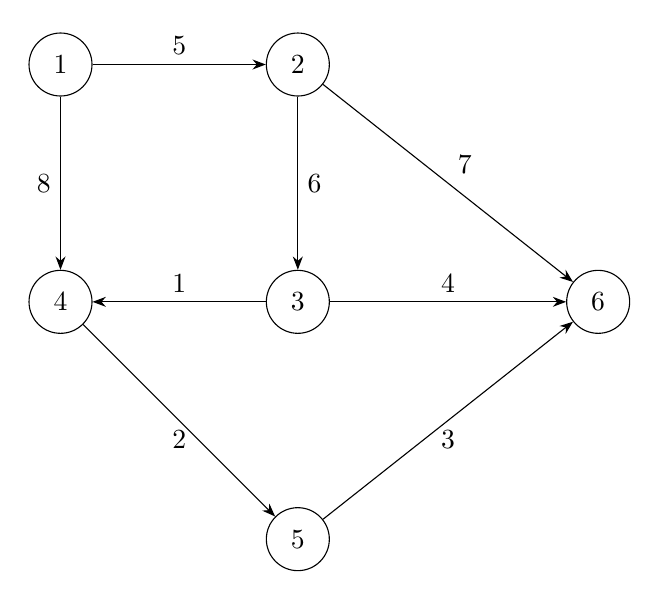
\begin{tikzpicture}[>=Stealth, node distance=22mm]
  \tikzset{v/.style={circle,draw,minimum size=8mm}}
  \node[v] (n1) {1};
  \node[v, right=of n1] (n2) {2};
  \node[v, below=of n2] (n3) {3};
  \node[v, below=of n1] (n4) {4};
  \node[v, below=of n3] (n5) {5};
  \node[v, right=30mm of n3] (n6) {6};

  \draw[->] (n1) -- node[above] {5} (n2);
  \draw[->] (n1) -- node[left] {8} (n4);
  \draw[->] (n2) -- node[right] {6} (n3);
  \draw[->] (n2) -- node[above right] {7} (n6);
  \draw[->] (n3) -- node[above] {1} (n4);
  \draw[->] (n3) -- node[above] {4} (n6);
  \draw[->] (n4) -- node[below] {2} (n5);
  \draw[->] (n5) -- node[below] {3} (n6);
\end{tikzpicture}
\caption{Q2 の有向重み付きグラフ}
\end{figure}

ダイクストラ法の更新過程を表に示す。ただし、$\infty$ は未到達を表す。

\begin{table}[h]
\centering
\caption{Q2 のダイクストラ法更新表}
\begin{tabular}{c|c|cccccc}
\toprule
Step & 確定頂点 & $d(1)$ & $d(2)$ & $d(3)$ & $d(4)$ & $d(5)$ & $d(6)$ \\
\midrule
初期 & -- & 0 & $\infty$ & $\infty$ & $\infty$ & $\infty$ & $\infty$ \\
1 & 1 & 0 & 5 & $\infty$ & 8 & $\infty$ & $\infty$ \\
2 & 2 & 0 & 5 & 11 & 8 & $\infty$ & 12 \\
3 & 4 & 0 & 5 & 11 & 8 & 10 & 12 \\
4 & 5 & 0 & 5 & 11 & 8 & 10 & 12 \\
5 & 3 & 0 & 5 & 11 & 8 & 10 & 12 \\
6 & 6 & 0 & 5 & 11 & 8 & 10 & 12 \\
\bottomrule
\end{tabular}
\end{table}

よって、1 から 6 への最短距離は、
\[
\boxed{12}
\]

であり、最短経路は以下の通りである。
\[
\boxed{1\to2\to6}
\]

\end{document}
